%%%%%%%%%%%%%%%%%%%%%%%%%
% Dokumentinformationen %
%%%%%%%%%%%%%%%%%%%%%%%%%
\newcommand{\titleinfo}{Physik 3 - Formelsammlung}
\newcommand{\authorinfo}{Braun \& Co, J.Rast, S.K\"orner, C.Gwerder}
\newcommand{\versioninfo}{$Version: 0.1$ | 
						gem\"ass Unterricht David Sourlier/HS2012}

%%%%%%%%%%%%%%%%%%%%%%%%%%%%%%%%%%%%%%%%%%%%%
% Standard projektübergreifender Header für
% - Makros 
% - Farben
% - Mathematische Operatoren
%
% DORT NUR ERGÄNZEN, NICHTS LÖSCHEN
%%%%%%%%%%%%%%%%%%%%%%%%%%%%%%%%%%%%%%%%%%%%%
% Genereller Header
\documentclass[10pt,twoside,a4paper,fleqn]{article}
\usepackage[utf8]{inputenc}
\usepackage[left=1cm,right=1cm,top=1cm,bottom=1cm,includeheadfoot]{geometry}
\usepackage[ngerman]{babel,varioref}

% Pakete
\usepackage{amssymb,amsmath,fancybox,graphicx,color,lastpage,wrapfig,fancyhdr,hyperref,verbatim}

%%%%%%%%%%
% Farben %
%%%%%%%%%%
\definecolor{black}{rgb}{0,0,0}
\definecolor{red}{rgb}{1,0,0}
\definecolor{white}{rgb}{1,1,1}
\definecolor{grey}{rgb}{0.3,0.3,0.3}
\definecolor{blue}{rgb}{0.2,0.2,0.9}

%%%%%%%%%%%%%%%%%%%%
% Generelle Makros %
%%%%%%%%%%%%%%%%%%%%
\newcommand{\kuchling}[1]{$_{\textcolor{red}{\mbox{\small{Kuchling #1}}}}$}
\newcommand{\stoecker}[1]{$_{\textcolor{grey}{\mbox{\small{Stöcker #1}}}}$}
\newcommand{\verweis}[2]{\small{(siehe auch \ref{#1}, #2 (S. \pageref{#1}))}}
\newcommand{\subsubadd}[1]{\textcolor{black}{\mbox{#1}}}

\newcommand{\grad}{\ensuremath{^\circ}}


\newcommand{\skriptsection}[2]{\section{#1 {\tiny Skript S. #2}}}
\newcommand{\skriptsubsection}[2]{\subsection{#1 {\tiny Skript S. #2}}}
\newcommand{\skriptsubsubsection}[2]{\subsubsection{#1 {\tiny Skript S. #2}}}


%%%%%%%%%%%%%%%%%%%%%%%%%%%%
% Mathematische Operatoren %
%%%%%%%%%%%%%%%%%%%%%%%%%%%%
\DeclareMathOperator{\sinc}{sinc}



% Fouriertransformationen
\unitlength1cm
\newcommand{\FT}
{
\begin{picture}(1,0.5)
\put(0.2,0.1){\circle{0.14}}\put(0.27,0.1){\line(1,0){0.5}}\put(0.77,0.1){\circle*{0.14}}
\end{picture}
}


\newcommand{\IFT}
{
\begin{picture}(1,0.5)
\put(0.2,0.1){\circle*{0.14}}\put(0.27,0.1){\line(1,0){0.45}}\put(0.77,0.1){\circle{0.14}}
\end{picture}
}



%%%%%%%%%%%%%%%%%%%%%%%%%%%%
% Allgemeine Einstellungen %
%%%%%%%%%%%%%%%%%%%%%%%%%%%%
%pdf info
\hypersetup{pdfauthor={\authorinfo},pdftitle={\titleinfo},colorlinks=false}
\author{\authorinfo}
\title{\titleinfo}

%Kopf- und Fusszeile
\pagestyle{fancy}
\fancyhf{}
%Linien oben und unten
\renewcommand{\headrulewidth}{0.5pt} 
\renewcommand{\footrulewidth}{0.5pt}

\fancyhead[L]{\titleinfo{ }\tiny{(\versioninfo)}}
%Kopfzeile rechts bzw. aussen
\fancyhead[R]{Seite \thepage { }von \pageref{LastPage}}
%Fusszeile links bzw. innen
\fancyfoot[L]{\footnotesize{\authorinfo}}
%Fusszeile rechts bzw. ausen
\fancyfoot[R]{\footnotesize{\today}}

% Einrücken verhindern versuchen
\setlength{\parindent}{0pt}

 
% Möglichst keine Ergänzungen hier, sondern in header.tex
\begin{document}
%%%%%%%%%%%%%%%%%%%%%%%%%%%%%%%%%%%%%%%%%%%%%%%%%%%%%%%%%%%%%%%%%%%%%%%%%%%%%%%%%%%%%%%%%%%%%%%%
%%%%%%%%%%%%%%%%%%%%%%%%%%%%%%%%%%%%%%%%%%%%%%%%%%%%%%%%%%%%%%%%%%%%%%%%%%%%%%%%%%%%%%%%%%%%%%%%
\section{Optik}

\subsection{Diverses}
\begin{tabular}{p{10cm}p{6cm}}
  \textbf{Wellenlängen der Spektralfarben} & \textbf{Konstanten} \\
  \begin{tabular}{|l|l|l|l|}
    \hline
      Wellenlänge in nm & Farbe & Wellenlänge in nm & Farbe \\
      \hline
      380 . . . 435 & violett  & 565 . . . 590 & gelb \\
      435 . . . 465 & blau     & 590 . . . 630 & orange \\
      465 . . . 485 & blaugrün & 630 . . . 780 & rot \\
      485 . . . 565 & grün & & \\
      \hline
  \end{tabular}
  & \textbf{Vakuumgeschwindigkeit:} \newline 
  $c=299'792'458 \frac{m}{s} \approx 3 \cdot 10^8 \frac{m}{s}$ \\
\end{tabular}

\subsection{Geometrische Optik \kuchling{360} \stoecker{309}}
\renewcommand{\arraystretch}{2}
\begin{tabular}{|p{3.5cm}|p{8.5cm}|p{6cm}|}
  \hline
  \begin{minipage}[]{3.5cm}
    Brechungsgesetz\\
    \kuchling{365} \stoecker{320}\\
  \end{minipage} &
  $\dfrac{\sin \varepsilon_1}{\sin \varepsilon_2} = \dfrac{n_2}{n_1} \qquad n_1
  \sin \varepsilon_1 = n_2 \sin \varepsilon_2 \qquad \varepsilon_1=\varepsilon_1'$ &
  \begin{minipage}[c]{5cm}
    \vspace{0.1cm}
    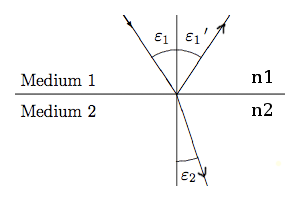
\includegraphics[width=4cm]{./bilder/Brechung.png}
  \end{minipage}\\
  \hline
  \begin{minipage}[]{3.5cm}
    \vspace{0.2cm}
    Brechungsindex\\
    \kuchling{365} \stoecker{320}\\
  \end{minipage}&
  $n=\dfrac{c}{u} \qquad$
  \begin{minipage}[]{4.5cm}
    [c]=Vakumgeschwindigkeit [u]=Lichtgeschwindigkeit
  \end{minipage} &
  \begin{minipage}[]{5cm}
    \renewcommand{\arraystretch}{1}
    \tiny
    \begin{tabular}{ l | l | l | l }
      & & & \\
      Medium & n & Medium & n \\
      \hline
      & & & \\
  		Luft   & 1,000292 & Kronglas (K13) & 1,522 \\
  		Wasser & 1,333    & Flintglas (K2) & 1,620 \\
      &          & Diamant        & 2,417 \\
    \end{tabular}
    \renewcommand{\arraystretch}{2}
  \end{minipage}\\
  \hline
  \begin{minipage}[]{3.5cm}
    Totalreflexion\\
    \kuchling{366} \stoecker{322}\\
  \end{minipage} &
  $\varepsilon = \arcsin \dfrac{n_1}{n_2} \quad$
  \begin{minipage}[]{6cm}
    $\varepsilon=\varepsilon_g \Rightarrow$ Grenzfall (ausgezogene Linie)
    $\varepsilon<\varepsilon_g \Rightarrow$ Brechung (gepunktete Linie)
    $\varepsilon>\varepsilon_g \Rightarrow$ Reflexion (gestrichelte Linie)     	
  \end{minipage} &
  \begin{minipage}[]{4cm}
    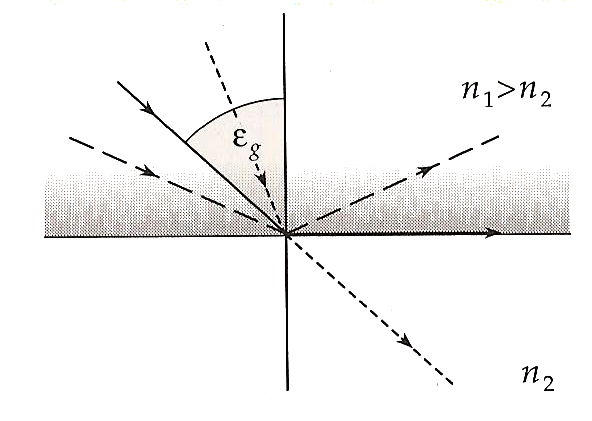
\includegraphics[width=3.5cm]{./bilder/Totalreflexion.png}
  \end{minipage}\\
  \hline
  \begin{minipage}[]{3.5cm}
    \vspace{0.2cm}
    Brennweite\\
    \kuchling{362} \stoecker{316}\\
  \end{minipage} &
  \begin{minipage}[]{6cm}
    Spiegel:\\
    $f=\dfrac{r}{2} \quad$ (für kleine $h$ gilt
    $a = b \approx \dfrac{r}{2}$) \\
    Linse:\\
    $\rightarrow$ Linsenschleifergleichung\\
  \end{minipage} &
  \begin{minipage}[]{6cm}
    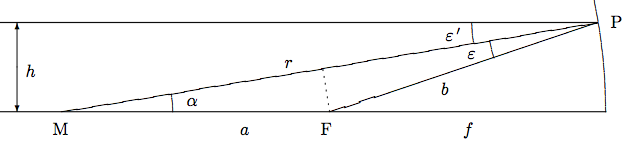
\includegraphics[width=6cm]{./bilder/BrennweiteSphaerischerSpiegel.png}
  \end{minipage}\\
  \hline
  \begin{minipage}[]{3.5cm}
    \vspace{2.7cm}
    Abbildungsgleichungen\\
    \kuchling{363} \stoecker{373}\\
  \end{minipage} &
  \begin{minipage}[c]{3cm}
    $\boxed{\dfrac{1}{f}=\dfrac{1}{g}+\dfrac{1}{b} \quad}$\\ \\
    $\boxed{\dfrac{B}{G}=\dfrac{b}{g}=\alpha}$ \\ \\
    $\boxed{\alpha_{tot} = \alpha_1 \cdot \alpha_2}$   
  \end{minipage}
  \begin{minipage}[c]{5cm}
    \vspace{0.2cm}
    G = Gegenstandshöhe\\
    g = Gegenstandsweite\\
    B = Bildhöhe\\
    b = Bildweite\\
    F = Brennpunkt\\
    f = Brennweite\\
    $\alpha$ = Vergösserungsfaktor \\
    $\alpha < 1$ = verkl., $\alpha > 1$ = vergr.\\
  \end{minipage}
  \begin{minipage}[]{8.5cm}
    \underline{Vorzeichenkonventionen}\\
    - Spiegel konkav bzw. Linse konvex $\quad \Rightarrow \quad f>0$\\
    - Spiegel konvex bzw. Linse konkav $\quad \Rightarrow \quad f<0$\\
    - Bild virtuell $\quad \Rightarrow \quad b<0 \quad\& \quad  B<0$\\
    - Gegenstand virtuell $\quad \Rightarrow \quad g<0 \quad \& \quad G<0$\\
  \end{minipage}&
  \begin{minipage}[]{6cm}
    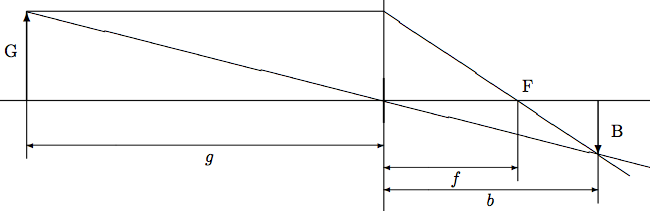
\includegraphics[width=6cm]{./bilder/Abbildungsgleichungen.png}
  \end{minipage}\\
  \hline
  \begin{minipage}[]{3.5cm}
    \vspace{0.2cm}
    Brechkraft,\\
    Linsenschleifergleichung\\
		\kuchling{370}\\
  \end{minipage} & 
  $D=\dfrac{1}{f}=\left(\dfrac{n_2}{n_1}-1\right)\left(\dfrac{1}{r_1}+
  \dfrac{1}{r_2}\right) \qquad D_{tot} = D_1 + D_2$ &
	\begin{minipage}[]{6cm}
		D = Dioptrien [dpt] \quad $1dpt=1m^{-1}$ \\
		$n_1$ = B.index d. umgebenden Mediums \\
		$n_2$ = B.index der Linse  
	\end{minipage} \\
	\hline
	Brillengleichung & $D_B = D'_{min} - D_{min} = 
	\frac{1}{g'_{min}} -\frac{1}{g_{min}}$ 
	& 
	\begin{minipage}[]{6cm}
	\vspace{0.1cm}
	 $D_B$: Dioptrien der Brille \\
	 $g'_{min}$:neue Entfernung zum Scharf sehen\\
	 $g_{min}$: alte Entfernung zum Scharf sehen \\
	 \vspace{0.1cm}
	\end{minipage} \\
	\hline
\end{tabular}

\renewcommand{\arraystretch}{1}
\newpage

\subsection{Spiegel \kuchling{362} \stoecker{315}}
\begin{minipage}[]{3.5cm}
  Konkavspiegel\\
  (Hohlspiegel)
\end{minipage}
\begin{minipage}[]{7cm}
  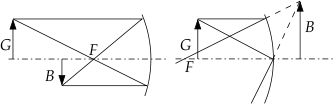
\includegraphics[width=6cm]{./bilder/Konkavspiegel.png}
\end{minipage}
\begin{minipage}[]{8cm}
  \small
  Gegenstand ausserhalb der Brennweite \\
  $\Rightarrow$ reelles, verkleinerte \& verkehrtes Bild \\ \\
  Gegenstand innerhalb der Brennweite \\
  $\Rightarrow$ virtuelles, vergrössertes \& aufrechtes Bild
\end{minipage}

\begin{minipage}[]{3.5cm}
  Konvexspiegel\\
  (Wölbspiegel)
\end{minipage}
\begin{minipage}[]{7cm}
  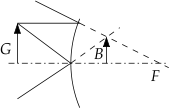
\includegraphics[width=3cm]{./bilder/Konvexspiegel.png}
\end{minipage}
\begin{minipage}[]{8cm}
  \small
  Gegenstand hat stets virtuelles, verkleinertes \& aufrechtes Bild
\end{minipage}

\begin{minipage}[]{3.5cm}
  Planspiegel
\end{minipage}
\begin{minipage}[]{7cm}
  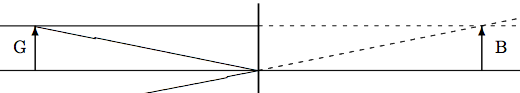
\includegraphics[height=1cm]{./bilder/Planspiegel.png}
\end{minipage}
\begin{minipage}[]{8cm}
  \small
  Bild ist virtuell und gleich gross wie Gegenstand, Bildweite ist gleich
  Gegenstandsweite. Brennpunkt liegt im Unendlichen.
\end{minipage}

\subsection{Linsen \kuchling{369} \stoecker{331}}
\begin{minipage}[]{3.5cm}
  Sammellinsen
\end{minipage}
\begin{minipage}[]{2cm}
  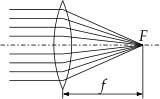
\includegraphics[width=2cm]{./bilder/sammelprinzip.png}
\end{minipage}
\begin{minipage}[]{5cm}
  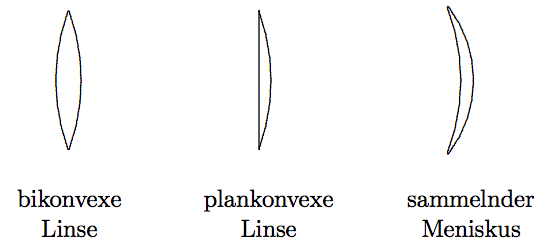
\includegraphics[width=5cm]{./bilder/sammellinsen.png}
\end{minipage}
\begin{minipage}[]{7.5cm}
  \small
  Gegenstand ausserhalb der Brennweite \\
  $\Rightarrow$ reelles, verkehrtes Bild \\ \\
  Gegenstand innerhalb der Brennweite \\
  $\quad \Rightarrow$ virtuelles, verkleinertes \& aufrechtes Bild
\end{minipage}

\begin{minipage}[]{3.5cm}
  Zerstreuungslinsen
\end{minipage}
\begin{minipage}[]{2cm}
  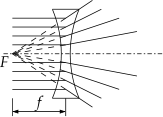
\includegraphics[width=2cm]{./bilder/streuprinzip.png}
\end{minipage}
\begin{minipage}[]{5cm}
  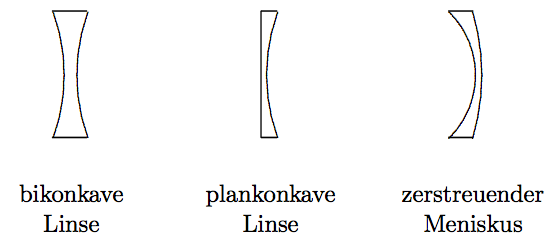
\includegraphics[width=5cm]{./bilder/streulinsen.png}
\end{minipage}
\begin{minipage}[]{7.5cm}
  \small
  Gegenstand hat stets virtuelles, aufrechtes \& verkleinertes Bild
\end{minipage}

\subsection{Abbildungsfehler}
\begin{tabular}{ll}
  Sph"arische Abberation & Brennweite ist Funktion des Abstands zur optischen
  Achse \\
  Koma & beim schiefen Einfall ($\rightarrow$ Schweiff"ormiger Fehler) \\
  Astigmatismus, Bildfeldw"olbung & vertikal und horizontal $\rightarrow$ andere
  Brennweite (Auge) \\
  Verzeichnung & tonnen- oder kissenf"ormige Verzeichnung eines Quadrates
  ($\rightarrow$ Photogrammetrie) \\
  Chromatische Abberation & wegen Dispersion $\Rightarrow$ Brennweite ist
  Funktion von $\lambda$ (Farbe) \\
\end{tabular}

\subsection{Optische Systeme}
\subsubsection{Kamera \kuchling{378} \stoecker{343}}
\begin{tabular}{lll}
  \parbox{3cm}{
    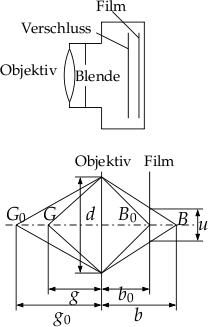
\includegraphics[width=3cm]{./bilder/kamera.png}} &
  \parbox{7cm}{
    Erzeugt reelles, verkleinertes \& umgekehrtes Bild \\
    \\
    $g \;$ Schärfentiefe\\
    $g_0 \;$ Eingestellte Entfernung (zum Gegenstand)\\
    $Z \;$ Blendenzahl \\
    $E \;$ Belichtung \\
    $u \;$ Unsch"arfekreisdurchmesser \\
    $q \;$ Öffnungsverhältnis (Blendenöffnung) \\
    $d \;$ Objektivdurchmesser \\
    $f \;$ Brennweite (z.B. 35mm-Objektiv)} &
  \parbox{8cm}{
    \fbox{$\dfrac{1}{g}=\dfrac{1}{g_0}\pm\dfrac{u}{q\,f^2}$} \\
    $B=\dfrac{f}{g-f}G$ \qquad bzw. f"ur $g\gg f\quad B=\dfrac{f}{g}G$\\
    $Z = \dfrac{f}{d} = \dfrac1q$ \qquad $q = \dfrac{d}{f} = \dfrac1Z$\\
    $E\sim q^2\,t$ \\
    Kleine Blende ($Z=16, \,q=1:16$)\\ 
    $\Rightarrow$ grosse Tiefensch"arfe\\
    Grosse Blende ($Z=4,\,q=1:4$) \\ 
    $\Rightarrow$ viel Licht, kleine Tiefensch"arfe} \\
\end{tabular}

\subsubsection{Lupe \kuchling{381} \stoecker{345}}
\begin{tabular}{lll}
  \parbox{7cm}{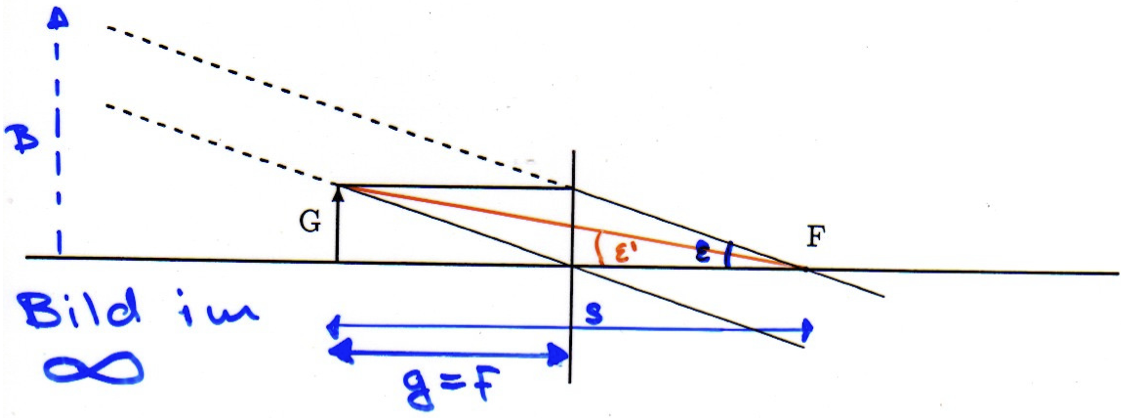
\includegraphics[width=7cm]{./bilder/lupe.png}} &
  \parbox{11cm}{
    Erzeugt virtuelles, vergrössertes \& aufrechtes Bild \\
    \\
    $V \;$ Vergr"osserung \qquad $s \;$ deutliche Sehweite (Auge: 25cm)\\
    \qquad $\varepsilon \;$ Sehwinkel mit \qquad $\varepsilon_0 \;$ Sehwinkel
    ohne Lupe \\
    \\
    $V=\dfrac{s}{f}=\dfrac{\tan(\varepsilon)}{\tan(\varepsilon_0)}\Rightarrow\dfrac{s}{g}>
    V_{\text{normal}}$ }
\end{tabular}
\subsubsection{Projektor \kuchling{377}}
\begin{tabular}{ll}
\parbox{6cm}{
  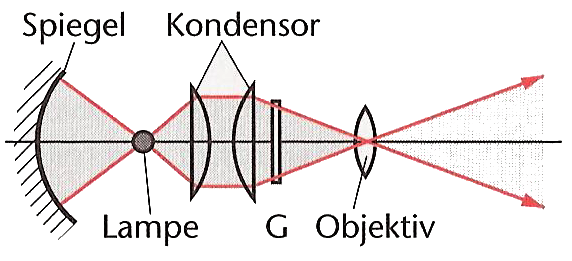
\includegraphics[width=6cm]{./bilder/projektor.png}} &
\parbox{12cm}{
  Erzeugt reelles, vergrössertes \& umgekehrtes Bild \\
  \\
  $\beta \;$ Abbildungsmasstab \\
  $\beta = \dfrac{b}{g} = \dfrac{b}{f}-1$}
\end{tabular}

\subsubsection{Mikroprojektor} 
Erzeugt reelles Bild auf Schirm mit $V=\dfrac{B}{G}=\dfrac{b}{g}$\\

\subsubsection{Mikroskop \kuchling{382} \stoecker{345}}
\begin{tabular}{ll}
  \parbox{8cm}{
    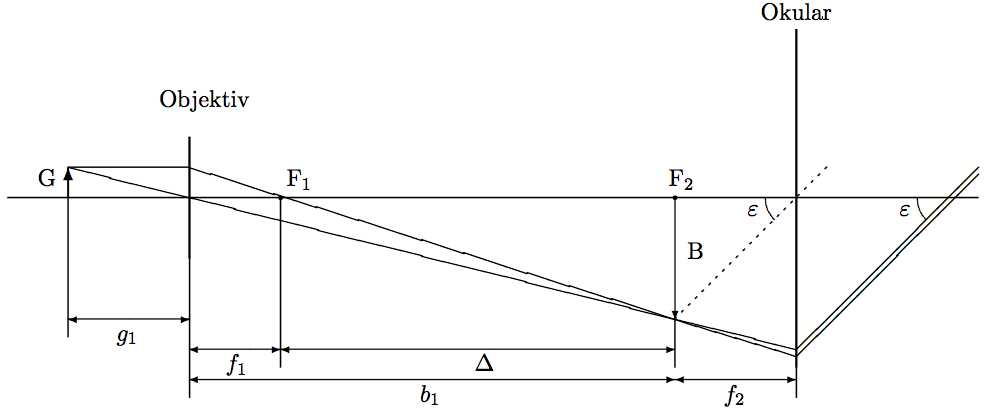
\includegraphics[width=8cm]{./bilder/mikroskop.png}} &
  \parbox{10cm}{
    Erzeugt reelles, vergrössertes \& umgekehrtes Bild. \\
    \\
    $V_1 = \frac{\Delta}{f_1} \;$ Vergrösserung des Objektivs\\
    $V_2 = \frac{s}{f_2} \;$ Vergrösserung des Okulars \\
    \\
    $\Delta = \overline{f_1\,f_2} \;$ Tubuslänge \\
    $V=V_1\,V_2= \dfrac{f_1}{f_2} = \dfrac{\Delta}{f_1} \dfrac{s}{f_2} =
    \dfrac{B}{G} \, \dfrac{s}{f_2}$ }
\end{tabular}

\subsubsection{Keplersches (Astronomisches) Fernrohr \kuchling{383} \stoecker{347}}
\begin{tabular}{ll}
  \parbox{11cm}{
    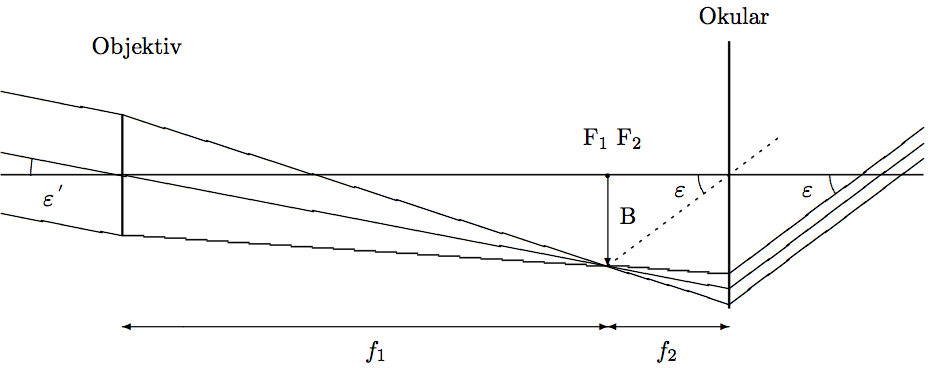
\includegraphics[width=10cm]{./bilder/astron.png}} &
  \parbox{7cm}{
    Erzeugt reelles, vergrössertes \& umgekehrtes Bild. Dies ist ein Spezialfall
    des Mikroskops, wo die \textbf{Gegenstandsweite} auf \textbf{unendlich} ($g \rightarrow \infty$) eingestellt ist. \\
    \\
    $D$ Durchmesser Objektiv \\
    $V$ Vergrösserung\\
    $a$ Abstand Okular-Austrittspupille\\
    $l$ Abstand Objektiv-Okular\\
    $d$ Grösse Austrittspup.\\
    $L$ Lichtstärke }
\end{tabular} \\
$V = \dfrac{\tan(\varepsilon)}{\tan(\varepsilon')} = \dfrac{B/f_2}{B/f_1} =
\dfrac{f_1}{f_2} = \dfrac{D}{d} = \dfrac{f_1+f_2}{a}$ \qquad $l = f_1+f_2$
\qquad $\dfrac{1}{f_1+f_2} + \dfrac{1}{a} = \dfrac{1}{f_2}$ \qquad
$a = \frac{l}{V} $ \qquad $d = \frac{D}{V}$ \qquad $L = d^2 = \left( \frac{D}{V}
\right)^2$

\subsubsection{Diverse \kuchling{384} \stoecker{347}}
\begin{tabular}{ll}
  Terrestr. Fernr. & 
  $V=\left|\dfrac{f_1}{f_2}\right|$ \qquad L"ange: $l=f-|f_2|$ (ent. mit
  Umkehrlinse (ZF), Prismen oder Streul. zur Umkehrung) \\
  Spiegelteleskope &
  Reflexion$\leftrightarrow$Brechung (weniger Lichtv.), k. Dispersion (k. chrom.
  Abberation), Verzug durch Masse  \\
\end{tabular}

\subsection{Konstruktion des Strahlengangs}
\begin{center}
  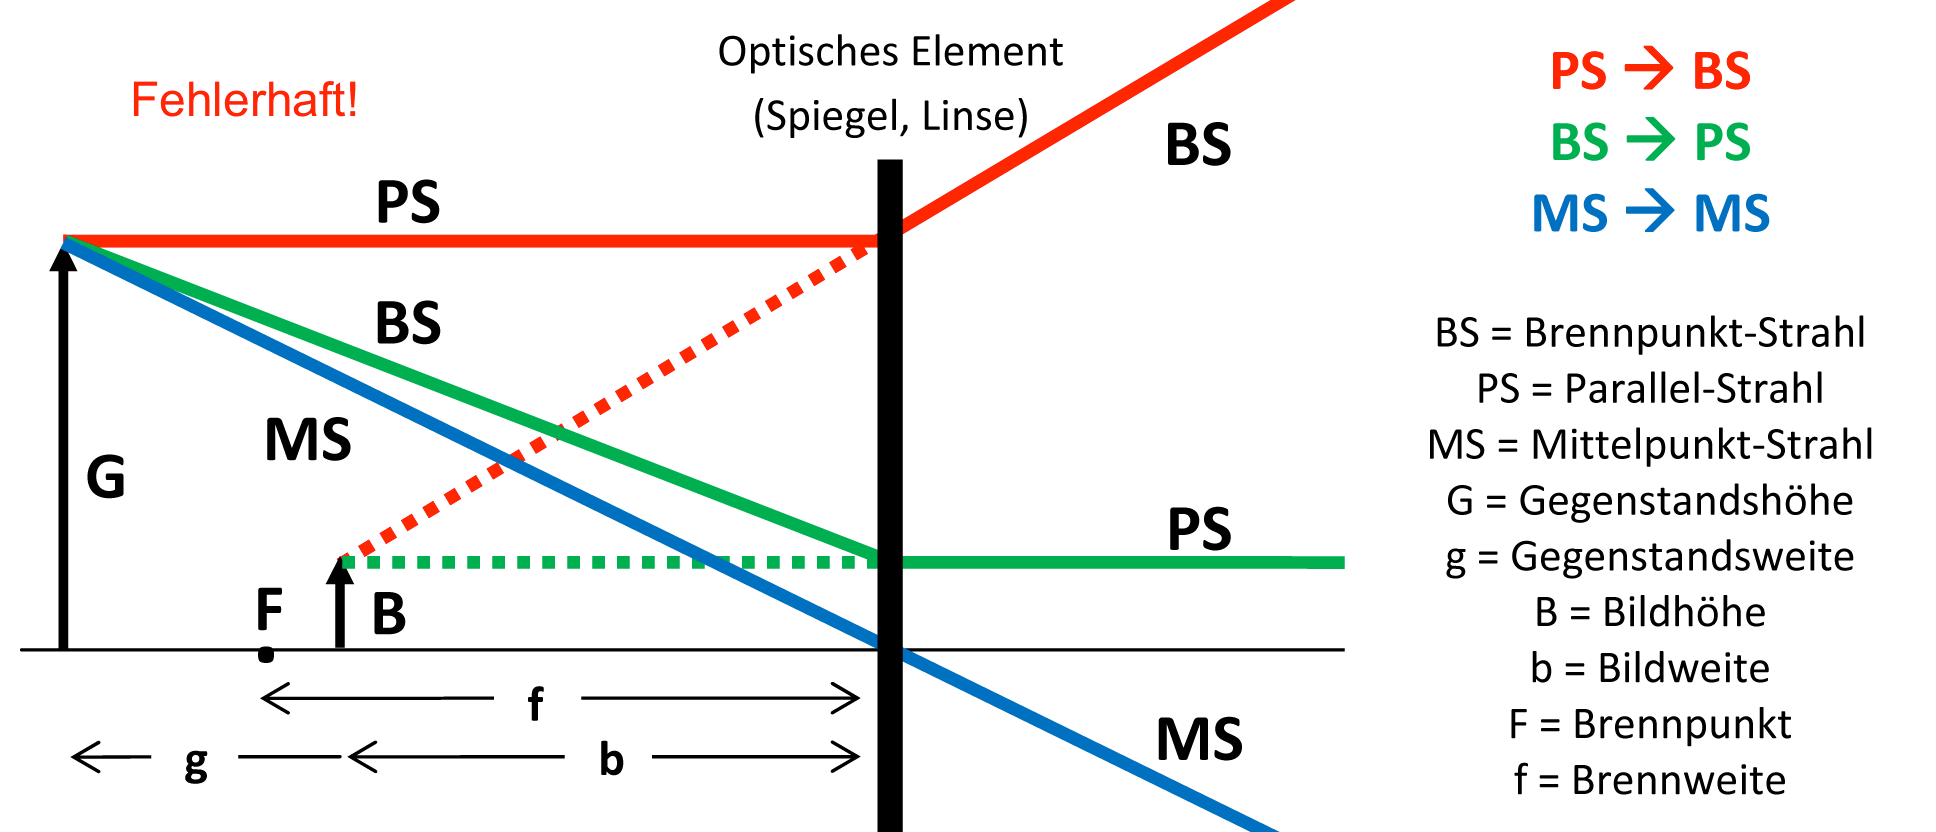
\includegraphics[width=11cm]{./bilder/strahlengang.png}
\end{center}


\section{Schwingungen \kuchling{192} \stoecker{235}}
\subsection{Ungedämpfte Schwingungen}
\renewcommand{\arraystretch}{2}
\begin{tabular}{|p{4cm}|p{8cm}|p{6cm}|}
	\hline
	\begin{minipage}[]{4cm}
    	Harmonische Schwingung\\
    	\kuchling{193} \stoecker{236}\\
    \end{minipage} &
	\begin{minipage}[]{8cm}
 		$y=A\,\sin(\omega t+ \varphi)  \qquad \omega=\dfrac{2\pi}{T}=2\pi f$\\ \\
		$\ddot{y}+\omega^2y=0 \qquad v(t)=\dot{y} \qquad a(t)=\ddot{y}$
    \end{minipage} &
	\begin{minipage}[]{6cm}
        \vspace{0.2cm}
 		$A$ = Amplitude $[1]$\\
 		$\omega$ = Kreisfrequenz $[\frac{1}{s}]$\\
 		$v(t)$ = Geschwindigkeit $[\frac{m}{s}]$\\
 		$a(t)$ = Beschleunigung $[\frac{m}{s^2}]$ 
     \end{minipage}\\
    \begin{minipage}[]{4cm} 
        	Trägheitskraft/Moment
    \end{minipage}&
    \begin{minipage}[]{8cm}
        	Trans. : $F_T(y) = m \cdot \ddot{y} \qquad$
        	Rot.: $M_T(\varphi) = J \cdot \ddot{\varphi}$
    \end{minipage} &\\
	\hline
	\begin{minipage}[]{4cm}
    	Schwingungsenergie\\
    	\kuchling{203} \stoecker{240}\\
    \end{minipage} &
	\begin{minipage}[]{8cm}
    \vspace{0.2cm}
	$E=E_{\text{pot}}+E_{\text{kin}}=\dfrac{c\,y^2}{2}+\dfrac{m\,v^2}{2}= \dfrac{c}{2}\cdot A$\\
	\\ $\dfrac{m\,\omega^2A^2}{2}(\sin(\omega t+\varphi)^2+\cos(\omega
	t+\varphi)^2)=\dfrac{m\,\omega^2\,A^2}{2}$\\
	\end{minipage} &
	\begin{minipage}[]{6cm}
		$E$ = Energie $[J]\\$
		$v=\dot y$ = Geschwindigkeit $[\frac{m}{s}]$\\
		$m$ = Masse $[kg]$\\	
    \end{minipage}\\
	\hline		
	\begin{minipage}[]{4cm}
    	Federpendel\\
    	\kuchling{198} \stoecker{238}\\
    \end{minipage} &
	\begin{minipage}[]{8cm}
    	\underline{ohne Federmasse:}\\
		$m\ddot{y}+c\,y=0 \qquad \omega_0=\sqrt{\dfrac{c}{m}} = \sqrt{\dfrac{c_1 +
		c_2}{m_1 + m_2}}$ \\ $T=2\pi \sqrt{\dfrac{m}{c}}$\\ \\
		rücktr. Kraft: $F=-cy=m\,\ddot{y} = F_T$ \\ \\
		\underline{mit Federmasse:}\\
		$\omega_0=\sqrt{\dfrac{c}{m+\frac{m_F}{3}}} \qquad
		T=2\pi\sqrt{\dfrac{m+\frac{m_F}{3}}{c}}$\\ 
		\end{minipage} &
	\begin{minipage}[]{6cm}
		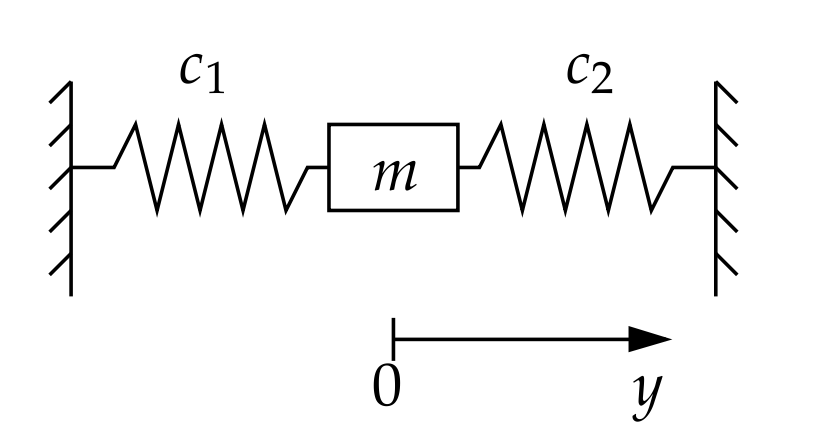
\includegraphics[width=3.5cm]{./bilder/Federpendel_masselos.png}\\ \\
		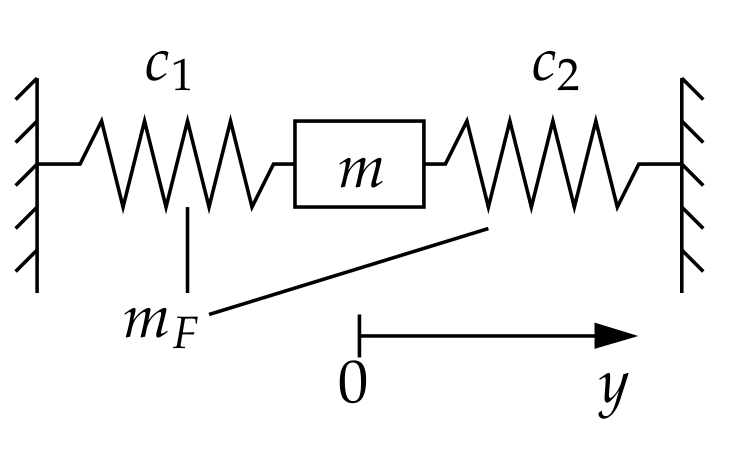
\includegraphics[width=3.5cm]{./bilder/Federpendel_masse.png}	\\		
    \end{minipage}\\
	\hline
	\begin{minipage}[]{4cm}
    	Drehpendel\\
    	\kuchling{199} \stoecker{245}\\
    \end{minipage} &
	\begin{minipage}[]{8cm}
	$J\ddot{\varphi}+c_{_D}\varphi=0 \qquad \omega_0=\sqrt{\dfrac{c_{_D}}{J}} \qquad
	T=2\pi\sqrt{\dfrac{J}{c_{_D}}}$\\ \\
	rücktr. Drehm.:	$M=-c_{_D}\,\varphi=J\,\ddot{\varphi}$ (Bewegung)\\
	\end{minipage} &
	\begin{minipage}[]{6cm}
    	\vspace{0.1cm}
		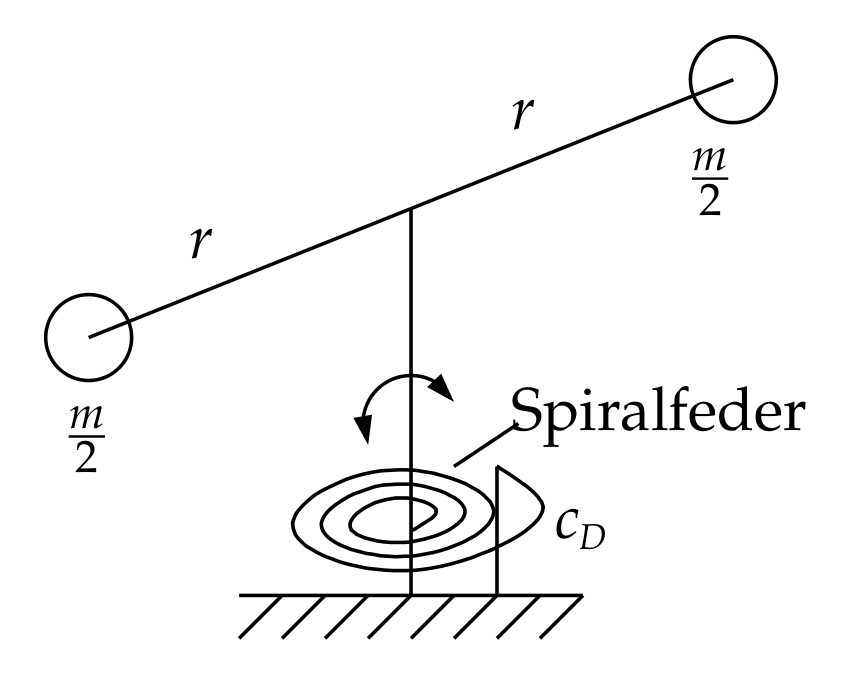
\includegraphics[width=3.5cm]{./bilder/Drehpendel.png}	
    \end{minipage}\\
	\hline
	\begin{minipage}[]{4cm}
    	Fadenpendel,\\
    	Mathematisches Pendel\\
    	\kuchling{200} \stoecker{240}\\
    \end{minipage} &
	\begin{minipage}[]{8cm}
	$l\ddot{\varphi}+g\sin(\varphi)=0\quad\xrightarrow{\text{lin.} (\varphi \ll 1)}\quad
	l\ddot{\varphi}+g\varphi=0$\\ \\
	$\omega_0=\sqrt{\dfrac{g}{l}} \qquad T=2\pi\sqrt{\dfrac{l}{g}} \qquad
	v=l\dot{\varphi} \qquad a=l\ddot{\varphi}$\\
	\end{minipage} &
	\begin{minipage}[]{6cm}
    	\vspace{0.1cm}
		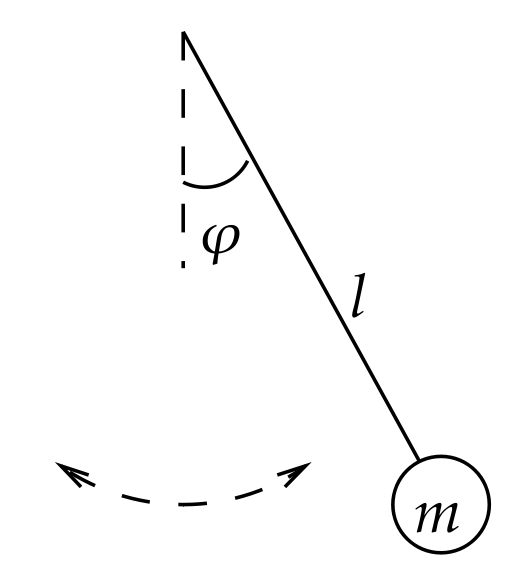
\includegraphics[width=2cm]{./bilder/mathe_pendel.png}	
    \end{minipage}\\
	\hline
	\begin{minipage}[]{4cm}
    	Physisches Pendel\\
    	\kuchling{201} \stoecker{243}\\ \\ \\
    	Massenträgheitsmomente\\
    	\kuchling{131} \stoecker{103}\\
    \end{minipage} &
	\begin{minipage}[]{8cm}
    \vspace{0.2cm}
	$J_A\ddot{\varphi}+m\,g\,a\sin(\varphi)=0$ $\xrightarrow{\text{lin.}}$ $
	J_A\ddot{\varphi}+m\,g\,a\,\varphi=0$\\ \\
	$\omega_0 = \sqrt{\dfrac{m\,g\,a}{J_A}}=\sqrt{\dfrac{g}{l^{*}}} \qquad
	T=2\pi\sqrt{\dfrac{J_A}{m\,g\,a}}=2\pi\sqrt{\dfrac{l^*}{g}}$\\ \\
	$l^{*}=\dfrac{J_A}{m\,a}=\dfrac{J_M}{m\,x} = \dfrac{J_{S}}{m\cdot a}+a$\\ 
	bei mehreren Elementen: \parbox{3cm}{
			$J_A = \sum J_{A_i}$\\
				 $m = \sum m_i$}\\ \\
	$J_A=J_S+m\,a^2 \qquad J_M=J_S+m\,x^2$\\ \\
	\textbf{Perkussionszentrum}\\
	Trifft ein Schlag den Schwingungsmittelpunkt $M$ wirken keine Kräfte auf den
	Punkt $A$ \& umgekehrt\\
	\textbf{Minimale Schwingungsdauer}\\
	$l_{min}^* = 2\sqrt{\dfrac{J_S}{m}}$ wenn $a=x=a_{min}$
	\end{minipage} &
	\begin{minipage}[]{6cm}
		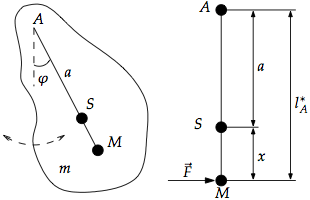
\includegraphics[width=6cm]{./bilder/physpendel.png}\\	
		\vspace{0.2cm}
		$\l^*$ = reduzierte Pendellänge\\
		$\l_A^* = l_M^*$
    \end{minipage}\\
	\hline
	\begin{minipage}[]{4cm}
    	Schwerpunkt berechnen\\
    	\kuchling{66} \stoecker{84}\\
    \end{minipage} &
	\begin{minipage}[]{8cm}
		$\vec{R}=\dfrac{\sum_i \vec{r_i} \Delta m_i}{m} \qquad m=\sum_i \Delta m_i$
	\end{minipage} &
	\begin{minipage}[]{6cm}
    	\vspace{0.2cm}
		$\vec{R}$ = Ortsvektor des Schwerpunkts\\
		$\vec{r_i}$ = Koordinate des $i$-ten Elements\\
		$\Delta m_i$ = Masse des $i$-ten Elements
    \end{minipage}\\
	\hline	
\end{tabular}
\renewcommand{\arraystretch}{1}

\subsection{Gedämpfte Schwingungen}
\renewcommand{\arraystretch}{2}
\begin{tabular}{|p{4cm}|p{8cm}|p{6cm}|}
	\hline
	\begin{minipage}[]{4cm}
    	Konstante Reibung\\
    	\kuchling{205} \stoecker{249}\\
    \end{minipage} &
	\begin{minipage}[]{8cm}
    	\vspace{0.2cm}
		$m\ddot{y}+cy+F_R=0 \qquad F_R=\mu\,F_N \qquad \Delta A=4\dfrac{F_R}{c} $\\
		Masse bleibt stehen, wenn $c\cdot A_n < F_R$
	\end{minipage} &
	\begin{minipage}[]{6cm}
        \vspace{0.2cm}
 		$\Delta A$ = Abnahme von $A$ pro Periode $[m]$\\
 		$F_R$ = Reibkraft $[N]$\\
 		$c$ = Federkonstante $[\frac{N}{m}]$\\ 
    \end{minipage}\\
	\hline
	\begin{minipage}[]{4cm}
    	Geschwindigkeitsprop. Dämpfung\\
    	\kuchling{205} \stoecker{250}\\
    \end{minipage} &
	\begin{minipage}[]{8cm}
	    \vspace{0.2cm}
	    \underline{$D<1$: Schwingfall}\\
		$m\,\ddot{y}+b\,\dot{y}+c\,y=\ddot{y}+\underbrace{\dfrac{b}{m}}_{2\delta}
		\cdot\dot{y}+\underbrace{\dfrac{c}{m}}_{\omega_0^{\,2}}\cdot y=0$\\
		$\qquad F_d=-b\dot y$\\ \\
		Ansatz abklingende Schwingung: \\
		$y(t)=A e^{-\delta t}\sin(\omega_d t+\varphi_0)$\\ \\
		$\delta=\dfrac{b}{2m}$\\
		$\omega_0=\sqrt{\dfrac{c}{m}}$ \\ 
		$\omega_d =	\omega_0 \sqrt{1-D^2} = \sqrt{\dfrac{c}{m}-\delta^2}=
		\sqrt{\omega_0^2 - \delta^2}$\\
		\\
		$\omega_r=\omega_0\sqrt{1-2\cdot D^2}$\\ \\
		$D=\dfrac{\delta}{\omega_0}=\dfrac{\frac{\Lambda}{2\pi}}{\sqrt{1+\left(\frac{\Lambda}{2\pi}\right)^2}} \approx \dfrac{\Lambda}{2\pi}$ (für kleine $D$)\\
		$\Lambda=\delta T=\dfrac{2\pi D}{\sqrt{1-D^2}}=\ln{\dfrac{\hat
		A_n}{\hat A_{n+1}}}\qquad\dfrac{\hat A_n}{\hat A_{n+1}}=e^{\delta T}$\\ 
		$\dfrac{A_{n+1}}{A_n} = \sqrt[\mathlarger{\mathlarger{k}}]{\dfrac{A_{n+k}}{A_n}}$\\ \\
		$\dfrac{E_t}{E_{t+\Delta t}}=\dfrac{A_t^2}{A_{t+\Delta t}^2} \qquad
		\dfrac{A_t}{A_{t+\Delta t}}= e^{\delta \Delta t} $\\ \\ \\
		\underline{$D>1$: Kriechfall (keine Schwingung mehr)}\\ \\
		$y(t)=b_1 e^{\lambda_1 t}+b_2e^{\lambda_2 t}$\\ \\
		$\lambda_1=-\omega_0(D+\sqrt{D^2-1})\quad\lambda_2=-\omega_0(D-\sqrt{D^2-1})$\\ \\
		\underline{$D=1$: Aperiodischer Grenzfall ($\delta = \omega_0$)}\\ \\
		$y=(b_1+b_2 t)\,e^{-\delta t} \qquad
		\omega_0^2=\dfrac{c}{m}=\dfrac{b^2}{4m^2}=\delta^2$\\
	\end{minipage} &
	\begin{minipage}[]{6cm}
 		$m$ = Mitschwingende Masse $[kg]$\\
 		$b$ = Dämpfungskonstante $[\frac{kg}{s}]$\\
 		$c$ = Federkonstante $[\frac{N}{m}]$\\
 		$F_d$ = Geschwindigkeits-proportionale Dämpfungskraft\\ \\
 		$\omega_0$ = Eigen-Kreisfr. $[\frac{1}{s}]$\\
 		$\omega_d$ = gedämpfte Kreisfr. $[\frac{1}{s}]$\\
 		$\omega_r$ = Resonanzkreisfrequenz $[\frac{1}{s}]$\\ \\ 				
 		$T$ = Periodendauer $[s]$\\
 		$A$ = Amplitude $[1]$\\
 		$\varphi_0$ = Phasenwinkel $[rad]$ \\ 		
 		$E$ = Energie $[J]$\\ \\
 		$\delta$ = Abklingkostante $[1/s]$\\
 		$D$ = Dämpfungsgrad $[1]$\\
		
 		$\Lambda$ = logartihmisches Dekrement $[1]$\\ \\
 		$\hat A_n$ = $A_{max}$ zu Zeitpunkt $t_n$ $[1]$\\
  		$\hat A_{n+1}$ = $A_{max}$ zu Zeitpunkt $t_n+T$ $[1]$\\
  		$E_t$ = $E$ zu Zeitpunkt $t$ $[J]$\\
  		$E_{t+\Delta t}$ = $E$ zu Zeitpunkt $t+\Delta t$ $[J]$\\
  		$A_t$ = $A$ zu Zeitpunkt $t$ $[1]$\\
  		$A_{t+\Delta t}$ = $A$ zu Zeitpunkt $t+\Delta t$ $[1]$\\	\\ \\ \\ \\ \\ \\
  		$b_1$ \& $b_2$ durch Anfangsbedingungen			
    \end{minipage}\\
	\hline	
\end{tabular}

\begin{multicols}{2}
\subsection{Diverse Formeln}
\begin{tabular}{|l|l||l|}
	\hline
	\textbf{Translation}	& \textbf{Rotation} & \textbf{Diverses}\\
	\hline
	\hline
	$x=$ Weg & $\varphi=$ Weg& 
	$F=m\cdot a$\\
	\hline
	$v=\dot{x}$ & $\omega=\dot{\varphi}$&
	$F=m\cdot\alpha\cdot r$\\
	\hline
	$a=\dot{v}=\ddot{x}$ & $\alpha=\dot{\omega}=\ddot{\varphi}$&
	$M=J\cdot\alpha=J\cdot\ddot{\varphi}$\\
	\hline
\end{tabular}

\subsection{Federn in Serie und Parallel}
\textbf{Parallel:} $c = c_1 + c_2$ \\
\textbf{Serie:} $ \frac{1}{c} = \frac{1}{c_1} + \frac{1}{c_2} \longrightarrow
c = \frac{c_1c_2}{c_1 + c_2}$
\end{multicols}
\newpage

\subsection{Fremderregte Schwingungen \kuchling{213} \stoecker{254}}
Die \textcolor{blue}{Erregungsschwingung} ist jeweils das Störglied der DGL.\\

\begin{tabular}{|l|l|}
\hline
\textbf{Allgemein}

	& \begin{minipage}[]{12cm}
      \renewcommand{\arraystretch}{2}      
		\begin{tabular}{lll}
    	Dimensionslose Frequenz
    		& $\eta=\dfrac{\omega}{\omega_0}$ 
			& $\omega$ = Erregerkreisfrequenz \\
    	Eigenkreisfrequenz
    		& $\omega_0 = \sqrt{\dfrac{c}{\sum m}}$
			& Federn parallel: $\omega_0 =
    		\sqrt{\dfrac{\sum c}{\sum m}}$
		\end{tabular} \\
    \end{minipage} \\
\hline
\hline
\parbox{6cm}{
	\textbf{Kraft- / Federkrafterregung}\\
	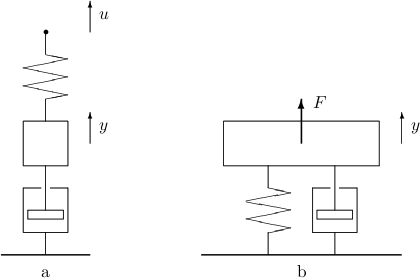
\includegraphics[width=6cm]{./bilder/federkrafterregung.png}}
	& \begin{minipage}[]{12cm}
      \renewcommand{\arraystretch}{2}      
		\begin{tabular}{ll}
    	Differentialgleichung
    		& $m \, \ddot{y} + b \, \dot{y} + c y=$
    		\textcolor{blue}{$c \, u_0 \, \sin(\omega t)$} \\
    	Amplitude
    		&
    		$A=\dfrac{c\,u_0}{m\sqrt{(\omega_0^2-\omega^2)^2+(2D\,\omega_0\,\omega)^2}}$ \\
    	Phase zw. $\omega_0$ \& $\omega$
    		&
    		$\varphi=\arctan\left(\dfrac{2D\,\omega_0\,\omega}{\omega_0^2-\omega^2}\right)$\\ 
    	Resonanzkreisfrequenz
    		& $\omega_r=\omega_0\sqrt{1-2D^2}$\quad $\omega_r<\omega_d<\omega_0$\\
    	Resonanzamplitude
    		& $A_r=\dfrac{u_0}{2D\sqrt{1-D^2}} = \dfrac{c \cdot u_0}{2m\sqrt{(\delta \omega_0)^2 - \delta^4}}$\\
    	Vergrösserungsfunktion
    		&
    		$V=\dfrac{1}{\sqrt{(1-\eta^2)^2+(2D\eta)^2}}=\dfrac{A(\omega)}{u_0}$ \\ 
    	Vergrösserung bei Resonanz
    		&
    		$V_r = \dfrac{1}{\sqrt{1-\eta_r^4}}$ mit $\eta_r = \sqrt{1-2D^2}$\\
    	\multicolumn{2}{l}{\parbox{12cm}{\small
    	Überkritische Dämfpung, wenn $D > \frac{1}{\sqrt2} \Rightarrow$ Auch bei 
    	Resonanz\\
    	bleibt Amplitude stets unter statischer
    	Auslenkung ($V \leq 1$)}}
		\end{tabular}
    \end{minipage} \\
\hline
\parbox{6cm}{
	\textbf{Indirekte Federkrafterregung}\\
	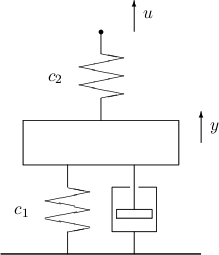
\includegraphics[width=4cm]{./bilder/indirekte-federkrafterregung.png}}
	& \begin{minipage}[]{12cm}
      \renewcommand{\arraystretch}{2}
		\begin{tabular}{ll}
    	Differentialgleichung
    		& $m \, \ddot{y} + b \, \dot{y} + c y=$
    		\textcolor{blue}{$c_2 \, u_0 \, \sin(\omega t)$} \\
    	Amplitude
    		&
    		$A=\dfrac{c_2}{c} 
    		\dfrac{c\,u_0}{m\sqrt{(\omega_0^2-\omega^2)^2+(2D\,\omega_0\,\omega)^2}}$ \\
    	Phase zw. $\omega_0$ \& $\omega$
    		&
    		$\varphi=\arctan\left(\dfrac{2D\,\omega_0\,\omega}{\omega_0^2-\omega^2}\right)$\\ 
    	Resonanzkreisfrequenz
    		& $\omega_r=\omega_0\sqrt{1-2D^2}$\\
    	Resonanzamplitude
    		& $A_r=\dfrac{u_0}{2D\sqrt{1-D^2}}$\\
    	Vergrösserungsfunktion
    		&
    		$V=\dfrac{c_2}{c}\cdot\dfrac{1}{\sqrt{(1-\eta^2)^2+(2D\eta)^2}}$
		\end{tabular}
    \end{minipage} \\
\hline
\parbox{6cm}{
	\textbf{Dämpferregung}\\ \\
	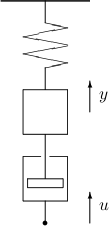
\includegraphics[width=2cm]{./bilder/daempferregung.png}}
	& \begin{minipage}[]{12cm}
      \renewcommand{\arraystretch}{2}
		\begin{tabular}{ll}
    	Differentialgleichung
    		& $m\,\ddot{y}+b\,\dot{y}+c\,y=$
    		\textcolor{blue}{$b\,\omega\,u_0\,\sin(\omega t+\frac{\pi}{2})$} \\
    	Amplitude
    		&
    		$A=\dfrac{b\,\omega\,u_0}{m\sqrt{(\omega_0^2-\omega^2)^2+(2D\,\omega_0\,\omega)^2}}$ \\
    	Phase zw. $\omega_0$ \& $\omega$
    		&
    		$\varphi=\operatorname{arctan}\left(\dfrac{2D\,\omega_0\,\omega}{\omega_0^2-\omega^2}\right)-\dfrac{\pi}{2}$\\ 
    	Resonanzkreisfrequenz
    		& $\omega_r=\omega_0 \quad \rightarrow$\quad max. bei $\eta=1$\\
    	Resonanzamplitude
    		& $A_r=u_0\quad\rightarrow\quad V(1)=1$\\
    	Vergrösserungsfunktion
    		&
    		$V=\dfrac{2 \,D\, \eta}{\sqrt{(1-\eta^2)^2+(2D\eta)^2}}$ 
		\end{tabular}
    \end{minipage} \\
\hline
\end{tabular}
\newpage
\begin{tabular}{|l|l|}
\hline
\parbox{6cm}{
	\textbf{Stützenerregung}\\ \\
	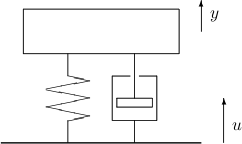
\includegraphics[width=4cm]{./bilder/stuetzenerregung.png}}
	& \begin{minipage}[]{12cm}
      \renewcommand{\arraystretch}{2}
		\begin{tabular}{ll}
    	Differentialgleichung
    		& $m\,\ddot{y}+b\,\dot{y}+c\,y=$
    		\textcolor{blue}{$c\,u_0\,\sin(\omega t) + b\,\omega\,u_0\,\cos(\omega t)$}
    		\\ & $m\, \ddot{q} + b\,\dot{q} + c\,q =$
    		\textcolor{blue}{$m\,\omega^2\,u_0\,\sin(\omega t)$} \\
    	Amplitude
    		&
    		$A=\dfrac{\omega^2\,u_0}{\sqrt{(\omega_0^2-\omega^2)^2+(2D\,\omega_0\,\omega)^2}}$ \\
    	Phase zw. $\omega_0$ \& $\omega$
    		&
    		$\varphi=\arctan\left(\dfrac{2D\,\omega_0\,\omega}{\omega_0^2-\omega^2}\right)-\pi$\\ 
    	Resonanzkreisfrequenz
    		& $\omega_r=\dfrac{\omega_0}{\sqrt{1-2D^2}}$\\
    	Resonanzamplitude
    		& $A_r=\dfrac{u_0}{2D\sqrt{1-D^2}}$\\
    	Vergrösserungsfunktion
    		& $V=\dfrac{\eta^2}{\sqrt{(1-\eta^2)^2+(2D\eta)^2}}$ 
		\end{tabular}
    \end{minipage} \\
\hline
\parbox{6cm}{
	\textbf{Unwuchterregung}\\ \\
	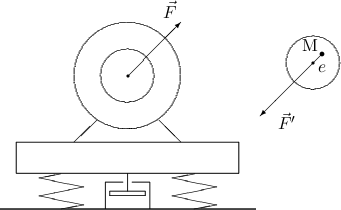
\includegraphics[width=6cm]{./bilder/unwuchterregung.png}\\ \\
	$m_R$ Rotormasse (bewegt)\\
	$e$ Exzentrizit"at (Distanz Achse$\leftrightarrow$SP) \\
	$F_0$ Kraft auf Fundament ohne Federung\\
	$F_{B0}$ verringerte Kraft}
	& \begin{minipage}[]{12cm}
      \renewcommand{\arraystretch}{2}
		\begin{tabular}{ll}
        $F(t)=F_0\cdot\sin(\omega t)$
        	& $F_0=m\cdot a_r=m\cdot\dfrac{v^2}{r}=m\cdot r\cdot \omega^2=m_R\cdot e \cdot \omega^2$ \\
    	Differentialgleichung
    		& $m\,\ddot{y}+b\,\dot{y}+c\,y=$
    		\textcolor{blue}{$m_R\,e\,\omega^2\,\sin(\omega t)$} \\
    	Amplitude
    		&
    		$A=\dfrac{m_R\,e\,\omega^2}{m\sqrt{(\omega_0^2-\omega^2)^2+(2D\,\omega_0\,\omega)^2}}$ \\
    	Phase zw. $\omega_0$ \& $\omega$
    		&
    		$\varphi=\operatorname{arctan}\left(\dfrac{2D\,\omega_0\,\omega}{\omega_0^2-\omega}\right)$\\ 
    	Resonanzkreisfrequenz
    		& $\omega_r=\dfrac{\omega_0}{\sqrt{1-2D^2}}$\\
    	Resonanzamplitude
    		& $A_r=\dfrac{m_R}{m}\dfrac{e}{2D\sqrt{1-D^2}}$\\
    	Kraftamplitude \textbf{ohne} Fed.
    		& $F_0 = m_R\,e\,\omega^2 \sin(\omega t)$\\
		Kraftamplitude \textbf{mit} Fed.
    		&
    		$F_{B0}=\dfrac{m_R\,e\,\omega^2\,\sqrt{1+4D^2\eta^2}}{\sqrt{(1-\eta^2)^2+4D^2\eta^2}}=F(\eta)$ \\ 
    	Verhältnis
    		&$\dfrac{F_{B0}}{F_0}=\sqrt{\dfrac{1+4D^2\eta^2}{(1-\eta^2)^2+4D^2\eta^2}}$ \\ 
		\end{tabular}
    \end{minipage} \\
\hline
\end{tabular}
\renewcommand{\arraystretch}{1}

\newpage

\subsection{Schwingkreise}
\subsubsection{Serienschwingkreis \kuchling{530} \stoecker{253}}
\renewcommand{\arraystretch}{2}
\begin{tabular}{|p{4cm}|p{14cm}|}
\hline
Diffgl: &
\begin{minipage}[]{14cm}
\vspace{0.2cm}
$L\ddot{I}+R_S\dot{I}+\dfrac{1}{C}\,I=\omega\,U_0\,\sin(\omega t +
\dfrac{\pi}{2})$ \qquad $I=I_0\,e^{-\delta t}\,\sin(\omega_d t+\varphi)$\\
\end{minipage}\\
\hline
Amplitude: &
\begin{minipage}[]{14cm}
\vspace{0.2cm}
$I_0=\dfrac{\omega\,U_0}{L\sqrt{(\omega_0^{\,2}-\omega^2)^2+(2D\,\omega_0\,\omega)^2}}$\\
\end{minipage}\\
\hline
Phase: &
\begin{minipage}[]{14cm}
\vspace{0.2cm}
$\varphi=\arctan{\dfrac{2D\,\omega_0\,\omega}{\omega_0^{\,2}-\omega^2}}-\dfrac{\pi}{2}$\\
\end{minipage}\\
\hline
Resonanzfrequenz: &
\begin{minipage}[]{14cm}
\vspace{0.2cm}
$\omega_r=\omega_0=\dfrac{1}{\sqrt{LC}}$ \qquad
$\omega_d=\omega_0\sqrt{1-D^2}=\dfrac{1}{\sqrt{LC}}\,\sqrt{1-\dfrac{R^2C}{4L}}$\\
\end{minipage}\\
\hline
Resonanzamplitude: &
\begin{minipage}[]{14cm}
\vspace{0.2cm}
$I_{0_r}=\dfrac{U_0}{R_S}$\\
\end{minipage}\\
\hline
Vergr"osserungsfunktion: &
\begin{minipage}[]{14cm}
\vspace{0.2cm}
$V(\eta)=\dfrac{\eta^2}{\sqrt{(1-\eta^2)^2+(2D\,\eta)^2}}$\qquad Max:
$V_m=\dfrac{1}{2D\sqrt{1-D^2}}$\\
\end{minipage}\\
\hline
Phasenverschiebung: &
\begin{minipage}[]{14cm}
\vspace{0.2cm}
$\varphi_U=\arctan\left(\dfrac{2D\,\eta}{1-\eta^2}\right)-\pi$\\
\end{minipage}\\
\hline
D"ampfungsgrad: &
\begin{minipage}[]{14cm}
\vspace{0.2cm}
$D=\dfrac{R_S}{2}\sqrt{\dfrac{C}{L}}$\\
\end{minipage}\\
\hline
Abklingkonst. : &
\begin{minipage}[]{14cm}
\vspace{0.2cm}
$\delta=\dfrac{R_S}{2L}$\\
\end{minipage}\\
\hline
\end{tabular}

\subsubsection{Parallelschwingkreis}
\begin{tabular}{|p{4cm}|p{14cm}|}
\hline
Diffgl: &
\begin{minipage}[]{14cm}
\vspace{0.2cm}
$C\ddot{U}+\dfrac{1}{R_P}\dot{U}+\dfrac{1}{L}U=\omega\,I_0\,\sin(\omega
t+\dfrac{\pi}{2})$\\
\end{minipage}\\
\hline
Amplitude: &
\begin{minipage}[]{14cm}
\vspace{0.2cm}
$U_0=\dfrac{\omega\,I_0}{C\sqrt{(\omega_0^{\,2}-\omega^2)^2+(2D\,\omega_0\,\omega)^2}}$\\
\end{minipage}\\
\hline
Phase: &
\begin{minipage}[]{14cm}
\vspace{0.2cm}
$\varphi=\arctan{\dfrac{2D\,\omega_0\,\omega}{\omega_0^{\,2}-\omega^2}}-\dfrac{\pi}{2}$\\
\end{minipage}\\
\hline
Resonanzfrequenz: &
\begin{minipage}[]{14cm}
\vspace{0.2cm}
$\omega_r=\omega_0=\dfrac{1}{\sqrt{LC}}$\\
\end{minipage}\\
\hline
Resonanzamplitude: &
\begin{minipage}[]{14cm}
\vspace{0.2cm}
$U_{0_r}=I_0\cdot R_P=\dfrac{\omega^2\,L^2}{R_S}$\\
\end{minipage}\\
\hline
Vergr"osserungsfunktion: &
\begin{minipage}[]{14cm}
\vspace{0.2cm}
$V(\eta)=\dfrac{1}{\sqrt{(1-\eta^2)^2+(2D\,\eta)^2}}$\qquad Max:
$V_m=\dfrac{1}{2D\sqrt{1-D^2}}$\\
\end{minipage}\\
\hline
Phasenverschiebung: &
\begin{minipage}[]{14cm}
\vspace{0.2cm}
$\varphi_I=\arctan\left(\dfrac{2D\,\eta}{1-\eta^2}\right)$\\
\end{minipage}\\
\hline
D"ampfungsgrad: &
\begin{minipage}[]{14cm}
\vspace{0.2cm}
$D=\dfrac{1}{2\,R_P}\sqrt{\dfrac{L}{C}}$\\
\end{minipage}\\
\hline
\end{tabular}
\renewcommand{\arraystretch}{1}

\subsubsection{G"ute}
$Q=2\pi\dfrac{E(t)}{E(t)-E(t+T)}=\dfrac{1}{2D}=V_m=\dfrac{\omega_0}{\Delta \omega}$\quad wobei \quad $E=\dfrac{C\,U^2}{2}+\dfrac{L\,I^2}{2}=\dfrac{L\,I_0^{\,2}}{2}=\dfrac{L\,\omega_0^{\,2}\,C^2\,U_0^{\,2}}{2}=\dfrac{C\,U_0^{\,2}}{2}$


\section{Wellen / Akustik \kuchling{229} \stoecker{265}}
\subsection{Definitionen räumlicher Elemtarwellen}
\begin{tabular}[]{|p{9cm}|p{9cm}|}
	\hline
	\begin{minipage}{9cm}
		\textbf{Wellengleichung:}\\
			$\ddot{\xi} = u^2 \cdot \xi''(x)$
	\end{minipage} &
	\begin{minipage}[]{9cm}
			$\ddot{\xi}$ = Zweite Ableitung nach der Zeit\\
			$\xi''$ = Zweite Ableitung nach dem Ort
	\end{minipage}\\
	\begin{minipage}[]{9cm}
    	\textbf{Ebene harmonische Welle:}\\
 		$\xi(\vec{r},t)=\xi_0 \sin(\omega t -k\vec{r}+\varphi)$\\ \\		   	
 		$\xi(\vec{r},t)=\xi_0 e^{-j(\omega t-k\vec{r})}$\\ \\ 
 		\textbf{Harmonische Kugelwelle:}\\
 		$\xi(\vec{r},t)=\dfrac{\xi_0}{|\vec{r}|} \sin(\omega
 		t-k|\vec{r}|+\varphi)$\\\\
 		$\xi(\vec{r},t)=\dfrac{\xi_0}{|\vec{r}|} e^{-j(\omega t-k|\vec{r}|)}$\\ 		
    \end{minipage} &
	\begin{minipage}[]{9cm}
    	\vspace{0.2cm}    
    	$\xi({\vec{r},t})$ = Auslenkung am Ort $\vec{r}$ zur Zeit $t$\\
		$\xi_0$ = Amplitude $[1]$\\
		$k$ = Wellenzahl $[\frac{1}{m}]$\\
		$\vec{r}$ = Ortsvektor $[m]$\\
		$\omega$ = Kreisfrequenz $[\frac{1}{s}]$\\
		$\varphi$ = Phasenverschiebung $[rad]$\\    
		$\lambda$ = Wellenlänge $[m]$\\
		$u$ = Wellengeschwindigkeit $[\frac{m}{s}]$\\
		$f$ = Frequenz $[Hz]$\\
		$T$ = Periodendauer $[s]$\\
    \end{minipage} \\
	\hline
\end{tabular}

\subsection{Wichtige Beziehungen}
$\boxed{k=\dfrac{\omega}{u}=\dfrac{2\pi}{\lambda}}$\quad
$\boxed{u=\dfrac{\omega}{k} = \lambda \cdot f}$ \quad
$\boxed{\lambda=\dfrac{2\pi}{k}=\dfrac{u}{f}}$ \quad
$\boxed{\omega=2\pi f=\dfrac{2\pi}{T}}$ \quad
$\boxed{f=\dfrac{\omega}{2\pi}=\dfrac{u}{\lambda}=\dfrac{1}{T}}$ \quad
$\boxed{T=\dfrac{1}{f}=\dfrac{2\pi}{\omega}}$ \quad
$\boxed{\varphi=\omega t-k|\vec{r}|}$

\subsection{Wellengeschwindigkeit \kuchling{233} \stoecker{267}}
\renewcommand{\arraystretch}{1.5}
\begin{tabular}{| p{6cm} | p{6cm} | p{6cm} |}
\hline
\textbf{Elastisch}e L"angs-/ Longitudinalwelle & \textbf{Elastisch}e Quer-/ Transversalwelle & Transversalwellen bei \textbf{Saite} oder Seil\\
$u=\sqrt{\dfrac{E}{\varrho}}$ & $u=\sqrt{\dfrac{G}{\varrho} }\quad$ mit $G=\dfrac{E}{2(1+\mu)}$ &
$u=\sqrt{\dfrac{F}{\varrho\,A}}=\sqrt{\dfrac{F}{\varrho}+\dfrac{\pi\,E\,A}{\varrho\,\lambda^2}}$
\\ $E$: Elastizit"atsmodul, $\rho$ = Dichte& $G$: Schubmodul, $\mu$ = Poisson-Zahl & $F$: Spannkraft, $E$:
Elastizit"atsmodul \\
\hline

Schwerewellen in \textbf{tiefem Wasser} & Schwerewellen in \textbf{flachem Wasser}& \textbf{Kapillarwellen}\\
$u=\sqrt{\dfrac{g\,\lambda}{2\pi}}$&$u=\sqrt{g\,h}$&$u=\sqrt{\dfrac{2\pi\,\sigma}{\varrho\,\lambda}}$\\
($\lambda \ll h$) & ($\lambda \gg h$)  & $\sigma$: Oberfl"achenspannung \\
\hline

Schallwellen in \textbf{Fluide}n & Schallwellen in \textbf{Gas}en & \textbf{Elektromagnetische} Wellen\\
$u=\sqrt{\dfrac{1}{\varrho\,\kappa}}$&$u=\sqrt{\dfrac{\varkappa\,p}{\varrho}}=\sqrt{\dfrac{\varkappa\,R\,T}{M}}$&
$u = \dfrac{c}{n}$\\
$\kappa$: Kompressibilit"at &$p$: Druck, $M$: Molmasse& n= Brechungsindex\\
& $\varkappa$: Adiabatenexponent&\\
\hline
\multicolumn{3}{|l|}{
	$M_{Luft}=
	0.02883 \dfrac{kg}{mol} = 28.83 \dfrac{g}{mol} \hspace{1.5cm}
	R=8.3145 \dfrac{J}{mol\cdot K} \hspace{1.5cm}
	\varkappa_{Luft}=1.4 \hspace{1.5cm}
	\text{T: }C^\circ+273,15K$
}\\
\hline
\end{tabular}
\renewcommand{\arraystretch}{1}

%\subsection{Stehende Welle}

%\begin{tabular}{|ll|lll|}
%	\hline
%	Laufzeit
%		& $ t = \dfrac{2\cdot l}{u} \qquad$
%		& \textbf{Intereferenzbedinung}
%		& $T_n = \dfrac{t}{n} = \dfrac{1}{n} \cdot \dfrac{2\cdot l}{u} \qquad$ 
%		& \parbox{6cm}{
%			$l$ = Länge des Objekts\\
%			$n$ = \textbf{ganzes} Vielfaches}\\
%	\hline
%\end{tabular}

\subsection{Eigenschwingungen Allg. /Akustik \kuchling{334} \stoecker{294}}
\renewcommand{\arraystretch}{2.5}
\begin{tabular}{|l|llll|}
\hline
\textbf{Allgemein}
	& Eigenfrequenz: 
	& $ f_n=\dfrac{1}{T_n} = n\cdot \dfrac{u}{2 \cdot l}$
	& Wellenlänge:
	& $\lambda_n=\dfrac{u}{f_n}=\dfrac{2\cdot l}{n}$\\
\hline
\textbf{Saiten}
	& Grundfrequenz: 
	& $ f_n= n \cdot \dfrac{1}{2l}\sqrt{\dfrac{F}{\varrho\,A}} = n \cdot \dfrac{1}{2l}\sqrt{\dfrac{\sigma}{\varrho}} $
	& 
	& $\lambda_n=\dfrac{2l}{n}$ \quad ($n=1,2,3,...$)\\
\hline
\textbf{Pfeifen} & Offen:
 	& $f_n=n\cdot \dfrac{1}{2l}\,u_{\text{Gas}}=n\cdot \dfrac{1}{2l}\sqrt{\dfrac{\varkappa\,R\,T}{M}}$ 
	& 
	& $\lambda_n=\dfrac{2l}{n}$ \quad ($n=1,2,3,...$)\\
& Gedeckt: 
 	& $ f_{(2n-1)}=\dfrac{2n-1}{4l}\sqrt{\dfrac{\varkappa\,R\,T}{M}}$
	& 
	& $\lambda_n=\dfrac{4l}{2n-1}$ \quad ($(2n-1)=1,3,5,...$) \\ 
\hline
\textbf{Membranen}
 	& &
 	$f_{mn}=\dfrac{1}{2}\sqrt{\dfrac{F}{\mu}}\sqrt{\dfrac{m^2}{a^2}+\dfrac{n^2}{b}}$ 
	& \multicolumn{2}{l|}{\parbox{8cm}{$m,n$: Anz. Oberwellen und $a,b$:
	L"ange/Breite \\
	$\mu$: Masse / Fläche; $F$: Spannkraft / Länge}} \\ \hline
\end{tabular}

\subsection{Doppler-Effekt \kuchling{342} \stoecker{277}}
\begin{tabular}{|l|l|l|}
\hline
\begin{minipage}[]{4cm}
		\small
		\vspace{.2cm}
		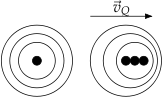
\includegraphics[width=3cm]{./bilder/doppler.png}\\
		Ruhende \& bewegte Punktquelle \\ \\ \\
		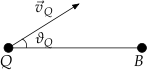
\includegraphics[width=3cm]{./bilder/doppler-bewegte-quelle.png}\\
		Bewegte Punktquelle \\ \\ \\
		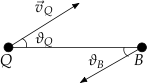
\includegraphics[width=3cm]{./bilder/doppler-beide-bewegt.png} \\
		Bewegter Beobachter \& bewegte Quelle \\
		\end{minipage}
	& \begin{minipage}[]{7cm}
      	\renewcommand{\arraystretch}{2}
      	\vspace{.2cm}
	  	\textbf{Bewegte Quelle, ruhender Beobachter} \\
	  	$f_B = \dfrac{1}{1 \mp  \dfrac{v_Q}{u}} f_Q$ \qquad \parbox{3cm}{- auf Hörer zu \\
	  				 + von Hörer weg}\\
	  	$f_B = \dfrac{1}{1 - \dfrac{v_Q}{u} \cos(\vartheta_Q)} f_Q$ \\
	  	\vspace{.5cm}\\
	  	\textbf{Ruhende Quelle, bewegter Beobachter} \\
	  	$f_B = \left(1 \pm \dfrac{v_B}{u}\right) f_Q$ \qquad + auf Quelle zu \\
	  	$f_B = \left(1 + \dfrac{v_B}{u} \cos(\vartheta_B)\right) f_Q$ \\
	  	\vspace{.5cm}\\
	  	\textbf{Allgemein} \\
	  	$f_B = \dfrac{u + v_B \cos(\vartheta_B)}{u - v_Q \cos(\vartheta_Q)} f_Q$ \\
	  	\vspace{.5cm}\\
	  	\textbf{Optischer (transversaler) Dop.-Effekt } \\
	  	$f_B = \dfrac{\sqrt{1 - \beta^2}}{1 - \beta \cos \vartheta_{rel}} f_Q \qquad \beta =
	  	\dfrac{v_{rel}}{c}$ \\ 
	  	$ \vec{v}_{rel} = \vec{v}_B - \vec{v}_Q \vspace{.5cm}\\
	  	\textbf{Schwebungsfrequenz}\\
	  	\Delta f = |f_{Empfangen} - f_{Gesendet}|$ \vspace{.2cm}
      	\renewcommand{\arraystretch}{1}
    	\end{minipage}
	& \parbox{6.5cm}{
		$f_B \;$ gehörte Frequenz \\
		$f_Q \;$ gesendete Frequenz \\
		$v_B \;$ Geschwindigkeit Beobachter \\
		$v_Q \;$ Geschwindigkeit Quelle\\
		$u \;$ Schallgeschwindigkeit\\
		$v_{rel} \;$ Relativgeschwindigkeit zw. Q und B\\
		$\vartheta_{rel} \;$ Winkel zwischen $\vec{v}_{rel}$ und $\overline{BQ}$
		} \\
\hline
\end{tabular}

\begin{minipage}{10cm}
	\subsection{Machscher Kegel \kuchling{344} \stoecker{278}}
	\begin{tabular}{ll}
	\parbox{5cm}{
		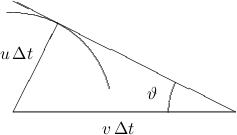
\includegraphics[width=4cm]{./bilder/machscher-kegel.png}}
		& 
		\parbox{5cm}{$\sin(\vartheta)=\dfrac{u}{v} = \dfrac{1}{M}$ \\ \\
		Machzahl: $M=\dfrac{v}{u}$}
	\end{tabular}
\end{minipage}
\begin{minipage}{8cm}
	\subsection{Lichtwellen}
		Lichtgeschwindigkeit: $ c = \dfrac{1}{\sqrt{\mu_0 \cdot \epsilon_0}} \qquad \qquad$ \\
		Intensität: $I = \dfrac{1}{2} \cdot \sqrt{\dfrac{\epsilon_0}{\mu_0}} \cdot {E_0}^2 \quad$ in $[W/m^2]$
\end{minipage}


\subsection{Optische Länge}
Durchqueren Wellen Medien, muss mit optischen Längen gerechnet werden.\qquad 
$s$ wird zu $n\,s$ \qquad $\lambda$ wird zu $\dfrac{\lambda}{n}$



\subsection{"Uberlagerung / Interferenz \kuchling{233, 235} \stoecker{272, 354}}
\setlength{\tabcolsep}{5pt}
\renewcommand{\arraystretch}{2}
\subsubsection{Interferenzbedingungen}
\begin{tabular}{p{11cm} p{7cm}}
\begin{minipage}[]{11cm}
	\begin{tabular}{|l|l|l|}
	\hline
	& \textbf{Phase} & \textbf{Weg} \\
	\hline
	Konstruktiv: 
		& $k_0(n\cdot \Delta x)=m \, 2\pi$
		& $n \, \Delta x = m \, \lambda$ \\
	Destruktiv: 
	 	& $k_0(n\cdot \Delta x)=(2m+1)\pi$
	 	& $n \, \Delta x = (2m+1) \frac{\lambda}{2}$ \\
	\hline
	\end{tabular}\\
	\end{minipage}
	& \parbox{8cm}{$k_0 = \dfrac{2\pi}{\lambda_0}$ = Wellenzahl im Vakuum\\
	$ \lambda_0$ = Wellenlänge im Vakuum\\
	n = Brechungsindex, Kuchling Tab 39, S.653\\
	$n\cdot \Delta x$ = optische Gangdifferenz}
\end{tabular}\\
\textbf{Phasensprung:}
		\parbox{16cm}{Ein Phasensprung um $\pi$ bzw. $\frac{\lambda}{2}$ findet bei
		\textbf{Reflektion} an einem härteren oder optisch dichterem Material
		(\textbf{höheres $n$}) statt.}
		
\subsection{Remission/Transmission}
\textbf{Remission} $R= \left(\dfrac{f-1}{f+2}\right)^2$ mit $ f = \dfrac{n_1}{n_2}$\hspace{2cm} \textbf{Transmission} $T = 1-R$  

\subsection{Schallmessung \kuchling{348} \stoecker{287}}
\setlength{\tabcolsep}{5pt}
\renewcommand{\arraystretch}{2.4}
\begin{tabular}{>{\bfseries}ll}
Welle: & $\xi=\xi_0\sin(\omega t-kx)$ \qquad $\xi_0$ Schallausschlag \qquad
$[\xi]$: m
\\
Schallschnelle: & $v=v_0\cos(\omega t-kx)\qquad\rightarrow\qquad v=\dot{\xi}=\omega\xi_0\cos(\omega t-kx)\rightarrow \dfrac{v_0}{\omega}=\xi_0$\\
Schall(wechsel)druck: & $\tilde p=\Delta p_0 \cos(\omega t-kx)$ \\
Druckamplitude: & $\Delta p_0=Z\cdot v_0$ \qquad Schallimpedanz $Z=\varrho
\cdot u$\\ 
Effektivwert: & $p_{\text{eff}} = \dfrac{\Delta p_0}{\sqrt{2}}$\\
Schallintensität: & $I=\dfrac{1}{2}\,\varrho\, v_0^{\,2}\,u =
\dfrac{1}{2}\varrho\,\omega^2\, \xi_0^{\,2}\,u =  \dfrac{\Delta
p_0^{\,2}}{2\cdot Z}$ \qquad $\xi_0$ Schallausschlag; $\varrho$ Dichte des Mediums\\  

Schallpegel [dB] : & $\boxed{L_I=10\cdot \log\left(\dfrac{I}{I_0}\right)}$\qquad
$I_0=10^{-12}$ W/m$^2$ \qquad $L_I=L_p$ f"ur Z=400kg/m$^2$s @ 20$^{\circ}$C\\
Schalldruckpegel: & $L_p=20\cdot\log\left(\dfrac{p_{\text{eff}}}{p_{\text{eff}_0}}\right)= 20\cdot\log\left(\dfrac{\Delta p_0}{\sqrt{2}\cdot p_{\text{eff}_0}}\right)$\qquad $p_{\text{eff}_0}=2\cdot 10^{-5}$ Pa\\
Schallschnellenpegel: & $L_v=20\cdot\log\left(\dfrac{v_{\text{eff}}}{v_{\text{eff}_0}}\right)$ \qquad $v_{\text{eff}_0}=5\cdot10^{-8}$m/s \\
Schallleistungspegel: & 
$L_P = 10\cdot\log\left(\dfrac{P}{P_0}\right)$ \qquad  $P_0=10^{-12}$W\\
Schallfluss: & $\vec q=\int\limits_{A}{\vec v\cdot dA}$\\
Wellengeschwindigkeit: & $u=\sqrt{\dfrac{1}{\varrho\,\kappa}}=\underbrace{\sqrt{\dfrac{\varkappa\,p}{\varrho}}=\sqrt{\dfrac{\varkappa\,R\,T}{M}}}_{\text{f"ur Gase}}$ \qquad (Schallgeschwindigkeit) $\kappa$: Kompressibilit"at \quad\\
& $\Rightarrow\dfrac{\Delta V}{V}=-\kappa\cdot\Delta p$ \qquad ($p\cdot V=\text{const}\,\,@\,\,T_{\text{const}}$ bzw. $p\cdot V^{\varkappa}=\text{const}$) \\
Lautstärke: & $S=2^{0.1\cdot(L_S-40)}$ \qquad $L_S=$ Lautst"arkepegel [phon] = $L_P$ @ 1kHz, H"orschwelle 4phon\\
Ebene Welle & (z.B. Parabolspiegel) $\rightarrow$ konstantes I, keine geom. D"ampfung nur Luftd"ampfung\\
& $\boxed{L_2=L_1-K\cdot(r_2-r_1)}$ f"ur $d<<r\quad\rightarrow\quad$ $I_2=\dfrac{P}{4\pi(r+d)^2}\approx\dfrac{P}{4\pi r^2}=I_1$\quad$I=$konstant\\
\parbox{3cm}{Kugelwellen\\
(Punktquellen)}: &  $I=\dfrac{P}{4\pi r^2}\quad\rightarrow\quad \sim\dfrac{1}{r^2}$ und $\dfrac{I_2}{I_1}=\dfrac{r_1^{\,2}}{r_2^{\,2}}$  \\
&$\boxed
{L_2=L_1-\underbrace{20\cdot\log\left(\dfrac{r_2}{r_1}\right)}_{\text{geom. D"ampfung}}-\underbrace{K\cdot(r_2-r_1)}_{\text{Luftd"ampfung}}}$\quad mit $K$: Schalldämpfung [dB/m]\\
\parbox{3cm}{Zylinderwellen\\
(Linienquellen)}: &$I=\dfrac{P}{l\,2\pi r}\quad\rightarrow\quad \sim\dfrac{1}{r} \quad \Rightarrow \boxed{L_2=L_1-10\cdot\log\left(\dfrac{r_2}{r_1}\right)-K\cdot(r_2-r_1)}$ \\
Schalld"ammung: & $\boxed{R=10\,\log\left(\dfrac{P_1}{P_2}\right)}$ \\
Phasensprung & um $\lambda/2$, $\pi$ bei Reflexion w"ahrend "Ubergang von gasf"ormig $\rightarrow$ fest  \\
Infra-/Ultraschall & Infraschall $<$ 16Hz...20kHz $<$ Ultraschall ...10GHz $<$ Hyperschall\\
\end{tabular}
\renewcommand{\arraystretch}{\arraystretchOriginal}

\subsection{Wellenoptik}

\subsubsection{Prinzip von Huygens \kuchling{229}}
Jeder Punkt einer Welle ist Zentrum einer neuen Kugelwelle  
(sogenannte Huygens‘sche Elementarwelle). 
Die Wellenfront zu einem späteren Zeitpunkt ist die Einhüllende dieser Huygens'schen Elementarwellen.\\

\begin{minipage}{9.5cm}
	\subsubsection{Beugung am Doppelspalt}
	\begin{minipage}{4.5cm}
	\textbf{Minimum n-ter Ordnung}\\
		$\sin(\varphi_n) \cdot s = (2n + 1)\cdot \frac{\lambda}{2} $\\
	\textbf{Maximum n-ter Ordnung}\\
			$\sin(\varphi_n) \cdot s = n \cdot \lambda $\\ 
			\\
		\begin{minipage}{4.5cm}
			$\lambda$ = Wellenlänge des Lichts\\
			$s$ = Spalt-Abstand\\
			$\varphi_n$ = Winkel n-ter Ordnung\\
			$n$ = 0,1,2,... = Ordnung
		\end{minipage}
	\end{minipage}
	\begin{minipage}{4cm}
		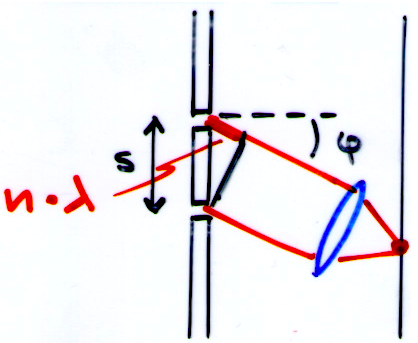
\includegraphics[width = 4cm]{./bilder/beugung-doppelspalt}
	\end{minipage}
\end{minipage}
\begin{minipage}{9cm}
	\subsubsection{Beugung am Einfachspalt}
	\begin{minipage}{4.5cm}
	\textbf{Minimum n-ter Ordnung}\\
		$\sin(\varphi_n) \cdot s = n \cdot \lambda $\\ 	
	\textbf{Maximum n-ter Ordnung}\\
		$\sin(\varphi_n) \cdot s = (2n + 1)\cdot \frac{\lambda}{2} $\\	
		\\
		\begin{minipage}{4.5cm}
			$\lambda$ = Wellenlänge des Lichts\\
			$s$ = Spalt-Abstand\\
			$\varphi_n$ = Winkel n-ter Ordnung\\
			$n$ = 0,1,2,... = Ordnung
		\end{minipage}
	\end{minipage}
	\begin{minipage}{4cm}
		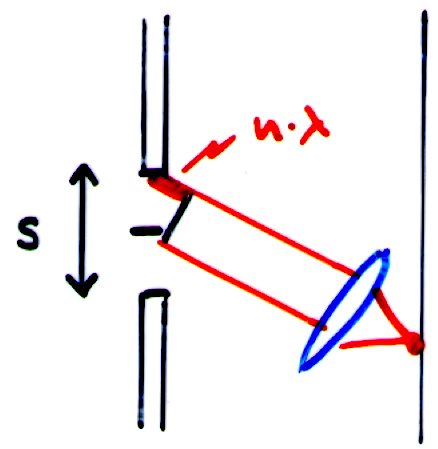
\includegraphics[width = 4cm]{./bilder/beugung-einfachspalt}
	\end{minipage}
\end{minipage}


\subsubsection{Beugung am Gitter}
\begin{minipage}{6cm}
	\textbf{Hauptmaximum n-ter Ordnung}\\
	$\boxed{\sin(\varphi_n) \cdot d = n \cdot \lambda}$\\
	\\
	\begin{minipage}{6cm}
		$\lambda$ = betrachtete Lichtwellenlänge\\
		$d$ = konstanter Spaltenabstand\\
		$\varphi_n$ = Maximumwinkel n-ter Ordnung \\
		$n$ = 0,1,2,... = Ordnung
	\end{minipage}
\end{minipage}
\begin{minipage}{5cm}
	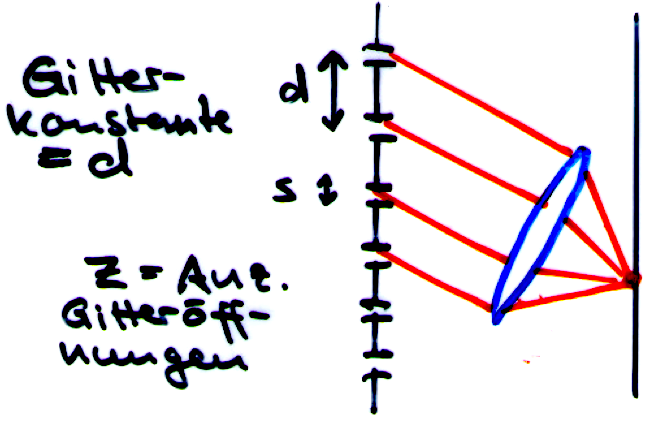
\includegraphics[width = 4cm]{./bilder/beugung-gitter}
\end{minipage}
\begin{minipage}{8cm}
	\textbf{Bedingungen für optimales optisches Gitter}
	\begin{enumerate}
		\item Möglichst kleine Gitterkonstante $\mathbf{d}$
		\item Möglichst grosse Gitter-Zahl $\mathbf{z}$
		\item Möglichst kleine Gitter-Breite $\mathbf{s}$
	\end{enumerate}
\end{minipage}\\
\\ \\
\begin{minipage}{18cm}
	\begin{tabular}{lllll}
	\parbox{4.5cm}{Intentitäts-Verteilung	\textbf{Gitter}}
		& $\approx$
		& \parbox{5.5cm}{Formfaktor\\
				{\small = Intensitätsverteilung \textbf{Einzelspalt}}}
		& $\times$
		& \parbox{6cm}{Interferenzfunktion\\
						{\small = Intensitätsverteilung \textbf{Doppelspalt}}}\\	
	\parbox{4.5cm}{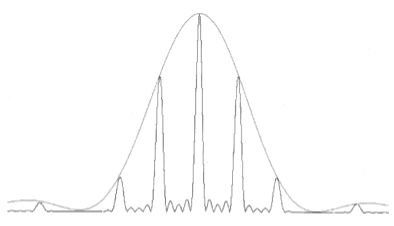
\includegraphics[width = 4.5cm]{./bilder/intensitaetsverteilung-gitter}}	
		& $\approx$
		& \parbox{4.5cm}{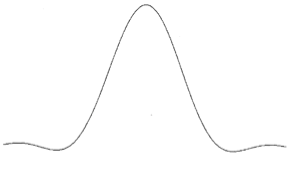
\includegraphics[width = 4.5cm]{./bilder/intensitaetsverteilung-einzelspalt}}
		& $\times$
		& \parbox{4.5cm}{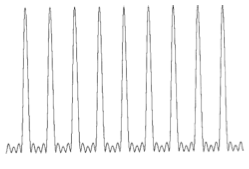
\includegraphics[width = 4.5cm]{./bilder/intensitaetsverteilung-doppelspalt}}
		\\			
	\end{tabular}
	Dabei entsteht immer z-2 Neben-Maxima.
\end{minipage}

\subsubsection{Babinet-Theorem}
Komplemetäre Strukturen (also Negativ und Positiv) liefern gleiche Beugungsbilder

\newpage


\section{Idiotenseite}
\input{idiotenseite/diverses/subsections/sivorsaetze}
\input{idiotenseite/trigo/subsections/Winkelargumente}
\input{idiotenseite/trigo/subsections/Periodizitaet}
\input{idiotenseite/diverses/subsections/pleite}

\subsection{Volumen}
\begin{tabular}{>{\bfseries}ll}
Kugel & $\frac{4}{3}\pi r^3$ \\
Zylinder & $\pi r^2 \cdot h$
\end{tabular}


\end{document}
